% last updated: 2020-08-04 Laci
%% toc-instructions.tex: Typesetting Guidelines for ToC
%% Requires toc.cls, tocbase.cls, and petersen.pdf in a directory that will be searched by 
%% LaTeX (LaTeX will automatically search the directory in 
%% which example.tex appears).
\documentclass{article}
\usepackage{fullpage}
\usepackage{listings}
\usepackage{amsmath,amsthm}
\usepackage{microtype}
\usepackage{hyperref,doi}
\usepackage{newtxtext}
\usepackage[cmintegrals]{newtxmath}
\usepackage{graphicx}
\usepackage{tikz}
\usepackage{caption,subcaption}
\usepackage{listings}
\usepackage[numbers]{natbib}
\usepackage{courier}

\lstset{language=[LaTeX]TeX,escapechar=|}
\lstset{basicstyle=\ttfamily,keywordstyle=\ttfamily}

\definecolor{gray}{gray}{0.5}

\newcommand{\eg}{e.\,g.}
\newcommand{\ie}{i.\,e.}
\newcommand{\phd}{\Ph.\,D.}
\newcommand{\bsc}{B.\,S.}
\newcommand{\msc}{M.\,S.}

\newcommand{\N}{\mathbb{N}}
\newcommand{\Z}{\mathbb{Z}}
\newcommand{\Q}{\mathbb{Q}}
\newcommand{\R}{\mathbb{R}}
\newcommand{\C}{\mathbb{C}}

\newtheorem{theorem}{Theorem}
\newtheorem{proposition}[theorem]{Proposition}
\newtheorem{definition}[theorem]{Definition}
\theoremstyle{plain}
\newtheorem{idea}[theorem]{Idea}
%\newtheorem{idea}{Idea}[section]

\newcommand{\expref}[2]{\texorpdfstring{\hyperref[#2]{#1~\ref{#2}}}{#1~\ref{#2}}}
\newcommand{\expeqref}[2]{\texorpdfstring{\hyperref[#2]{#1~\eqref{#2}}}{#1~\eqref{#2}}} 

\DeclareMathOperator{\Schur}{\mathbb{S}}
\DeclareMathOperator{\Specht}{Specht}
\DeclareMathOperator{\cov}{\textsl{Cov}}

\theoremstyle{definition}
\newtheorem{thought}[theorem]{Thought}
%\newtheorem{thought}{Thought}[section]

\hypersetup{colorlinks=true,breaklinks,anchorcolor=blue,linkcolor=blue,urlcolor=gray,citecolor=blue}

\begin{document}
\title{Typesetting Guidelines for the\\ \textsl{Theory of Computing}}

\maketitle

\begin{abstract}
  This document describes \LaTeX\ typesetting guidelines for the
  \emph{Theory of Computing}, including the use of the
  \texttt{toc.cls} class file.
\end{abstract}

\begin{center}
\Large{\textsc{Primer}}
\end{center}

While detailed instructions for using the ToC\TeX\ packages appear in
the complete guide below, in most cases you may typeset your article by
adapting the template file \lstinline`toc-template.tex` and adhering to the
following basic guidelines.
\begin{enumerate}
\item Please submit your manuscript in a single \texttt{.tex} file and a
     single \texttt{.bib} file, plus the figure files.  Copyediting
     becomes extremely cumbersome when the article is divided
     up into multiple source files.
\item Minimize usage of \LaTeX\ packages and elaborate \LaTeX\
  macros.  Please delete all macros not used in the paper.
\item \emph{Never} use \lstinline.\def. to define commands; instead use the
  robust command \lstinline.\newcommand..  All author-defined
  macros must have names that are \emph{at least three characters},
  to avoid conflict with predefined macros.
  \emph{Do not use} \lstinline.\renewcommand. as it will, by design,
  change the meaning of predefined macros and may cause 
  typesetting errors that will go undetected.
\item
  Please remove all text from the source file that does not contribute
  to the PDF output.  This includes text made invisible by various
  constructs such as \lstinline'\iffalse ... \fi' or \lstinline'\ignore{...}'.
  The reason for this request is twofold: these invisible passages
  considerably increase the copy editors' job; and they remain visible
  in the final published source file.  They can also be a source of
  big potential mistakes.

  \emph{Exception:} Do not remove the text of our template,
     but please remove your own text commented out 
     by \lstinline'%' signs to help the copyeditor.

  \emph{Note:}
     All commented-out text will be automatically removed
     before publication.
\item If a preliminary version of your article has been published, add
  a footnote to the title with a reference to the preliminary
  version. If possible, link to the preliminary version, preferably
  with a DOI. For example:
\begin{lstlisting}
\title{Article title\titlefootnote{A
   \href{http://dx.doi.org/10.1145/1806689.1806743}{preliminary
   version} of this paper appeared in the Proc. of the 42nd ACM
   Symp.\ on Theory of Computing (STOC'10).}}
\end{lstlisting}
Note that links to DOIs have the form
\lstinline,http://dx.doi.org/,\textsl{(doi)}. Thus
\begin{lstlisting}
http://dx.doi.org/10.1145/1806689.1806743
\end{lstlisting}
is the proper link to the DOI
\lstinline,10.1145/1806689.1806743,.

\item Your abstract should be self-contained. Please refer to
citations by author name rather than number. For example, rather than
\begin{center}
  \parbox{5in}{This paper continues the work of [8] and builds upon
  the techniques of [17] and [18].}
\end{center}
we prefer
\begin{center}
\parbox{5in}{This paper continues the authors' work (ICALP'05) and builds upon the
techniques of Taylor et al.\ (2005) and Taylor and Zhang (STOC'04).}
\end{center}
Here ``Taylor et al.'' refers to a journal article with three or more
authors.
\item We prefer to place tiny spaces between the letters in
  abbreviations like Ph.\,D., M.\,S., e.\,g., i.\,e., etc. This can be
  accomplished in \LaTeX\ using \lstinline.\,., which produces a small
  space; thus,
  \begin{center}
    \lstinline!Ph.\,D.!\qquad \lstinline!M.\,S.! \qquad \lstinline!B.\,S.! \qquad \lstinline!e.\,g.!\qquad\ldots
  \end{center}
  We supply the macros \lstinline!\phd!, \lstinline!\msc!, \lstinline!\bsc!,
  \lstinline!\eg!, and \lstinline!\ie!, which will produce these abbreviations
  with correct spacing. Note that in standard usage, the abbreviations
  ``\eg'' and ``\ie'' are always followed by a comma.
\item
  Please use \lstinline'\emph' rather than \lstinline'\em' to \emph{emphasize}
  text, as \lstinline'\emph' is smart about space following the emphasized
  text: the emphasized text ``\emph{sonticus}'' is produced with the
  \LaTeX\ fragment \lstinline'\emph{sonticus}'. Similarly, use the \LaTeX2e commands \lstinline'\texttt',
  \lstinline'\textsl', \lstinline'\textit', \lstinline'\textsf', and \lstinline'\textbf',
  to produce \texttt{teletype}, \textsl{slanted}, \textit{italic},
  \textsf{sans-serif}, and \textbf{bold} text. These commands take the
  text on which they operate as arguments: thus
  \lstinline'\textsf{sans-serif}' produces \textsf{sans-serif}.
  In math mode, please use the \lstinline,\text, command to produce
  fragments of regular text. For example,
\begin{lstlisting}
\[
C_U = \{ f \mid \text{$f$ is uniformly continuous on $U$}\}
\]
\end{lstlisting}
  produces the typesetting
  \[
  C_U = \{ f \mid \text{$f$ is uniformly continuous on $U$}\}
  \]

  Use \lstinline'\N', \lstinline'\Z', \lstinline'\Q', \lstinline'\R',
  and \lstinline'\C' to produce the symbols for the five common number
  systems; they will be typeset in blackboard-bold as $\N$, $\Z$,
  $\Q$, $\R$, $\C$.  Use the \lstinline'\mathbb' command to create other
  blackboard-bold characters in math mode; for instance
  \lstinline'\mathbb{H}' will produce $\mathbb{H}$, the standard symbol for
  the quaternions.

\item You are probably familiar with \LaTeX's mechanism for labels and
  references (via the \lstinline,\label, and \lstinline,\ref,
  commands). In ToC articles, we use an amplification of this system
  offered by the \lstinline,\expref, command. The advantage is that
  this command provides a larger hyperlink anchor: for example, the
  standard reference \lstinline,Theorem~\ref{thm:Markov}, produces the
  typesetting Theorem~\ref{thm:Markov}; note that the number is the
  anchor. In contrast, the command
  \lstinline,\expref{Theorem}{thm:Markov}, produces the typesetting
  \expref{Theorem}{thm:Markov}. Please use \lstinline,\expref, where
  you would usually use \lstinline,\ref, with the exception of
  equations, which are referred to with the \lstinline`\expeqref`
  command: \eg, \lstinline`\expeqref{equation}{eq:covariance}` which
  produces the typesetting: \expeqref{equation}{eq:covariance}.

\item Macros for theorem-like environments (theorems, definitions,
  etc.) and proofs are provided by \lstinline`toc.cls` (using the
  \lstinline`amsthm` package). Theorems, propositions, definitions, etc.,
  are typeset via the familiar evironments:
\begin{lstlisting}
\begin{theorem}[Stokes' Theorem]
  Theorem body.
\end{theorem}
\end{lstlisting}
Proofs are typeset similarly:
\begin{lstlisting}
\begin{proof}
  Proof body.
\end{proof}
\end{lstlisting}
In cases where a proof \emph{ends} with a displayed equation, use the
\lstinline,\qedhere, command to place the end of proof marker on the same
line as the displayed equation. For example,
\begin{lstlisting}
\begin{proof}
  ...
  And we conclude that
  \[
  X = \iint_{\delta S} f\,. \qedhere
  \]
\end{proof}
\end{lstlisting}
will produce
\begin{proof}
  \dots\\
  We conclude that
  \[
  X = \iint_{\delta S} f\,. \qedhere
  \]
\end{proof}
(Without the \lstinline,\qedhere, command, the $\Box$ symbol would appear on
the following line.) When a proof is presented without a proof
environment, use the \lstinline.\qed. command to manually lay out an ``end
of proof'' marker: \qed


In the case where a proof is not adjacent with the theorem it
supports, indicate this with the optional argument as below:
\begin{lstlisting}
\begin{proof}[Proof of \expref{Theorem}{thm:Markov}.]
  To prove inequality~\eqref{markov.eq}, expand the definition of
$E[X]$.
\end{proof}
\end{lstlisting}
This produces the typeset output:
\begin{proof}[Proof of \expref{Theorem}{thm:Markov}.]
  To prove inequality~\eqref{markov.eq}, expand the definition of
$E[X]$.
\end{proof}
See \expref{Section}{sec:math} for further details.
\item ToC numbers theorems, lemmas, definitions, remarks, etc.
  consecutively within each section.  So Section 3 might begin with
  Definition 3.1, followed by Theorem 3.2, Remark 3.3, Lemma 3.4,
  Theorem 3.5, etc.  \emph{Please do not defeat this numbering system.}
\item Make sure you use the math operators provided by LaTeX, \eg,
  \lstinline.\log., \lstinline$\ln$, \lstinline$\exp$, \lstinline$\dim$, \lstinline$\min$,
  \lstinline$\max$. These will result in appropriate type and spacing.
 If you need to define your own operator, use the
\lstinline$\DeclareMathOperator$
command in the preamble (before \lstinline$\begin{document}$).
For example,
\begin{lstlisting}
\DeclareMathOperator{\Schur}{\mathbb{S}}
\DeclareMathOperator{\Specht}{Specht}
\begin{document}
...
Schur-Weyl duality yields $V^{\otimes n} = \bigoplus_\lambda
(\Schur^\lambda(V)) \otimes \Specht_\lambda$.
\end{lstlisting}
will print ``Schur-Weyl duality yields $V^{\otimes n} = \bigoplus_\lambda
(\Schur^\lambda(V)) \otimes \Specht_\lambda$.''

\item  Please use the ToC macro 
\lstinline.\eee. to typeset the base of the natural logarithm.
This will print \lstinline.\mathrm.  ``$\mathrm{e}$''
to distinguish it from variables that might be called \emph{e}.
\item Graphics must be supplied in \lstinline`.pdf` (acrobat) and included
with the \lstinline`\includegraphics` command. We encourage use of
pgf/Ti$k$Z for creation of in-line graphics. We use the
\lstinline.subcaption. package to layout subfigures. See
\expref{Section}{sec:figures} for a more complete description.
\item Supply your cited references as a Bib\TeX\ database.
\item ToC publishes reasonably full names of bibliography
  authors.  Please supply them.
\item It will be most helpful if you can provide
    \emph{include digital
    object identifiers} for each Bib\TeX\ record. This
    amounts to adding, for each Bib\TeX\ record, a line of the form
\begin{lstlisting}
   doi = {xxx},
\end{lstlisting}
  See \expref{Section}{sec:bibliography} for further details.
\item ToC discourages appendices.  We ask you to fold their
material into the body of the article. If you feel some
material must remain in appendices, please place those appendices
before the acknowledgments and the biblography.
\item ToC posts authors' photos on the ``About the authors'' web page
associated with the article. If you agree to have your picture posted,
please email it to the editors in jpeg format, along with the final,
ToC-typeset manuscript. Ideally the picture
should be 150 pixels wide; if it is different, the software will
adjust its width to 150 pixels. The height to width ratio of the
picture should be between $2^{1/\pi}$ and the golden ratio: an ideal
photograph will be $150 \times 243$ pixels.
\item Please include a brief biographic sketch of each author at the
end of the article, in the ``about the authors'' section. Take the
biographical
sketches of previously published papers as models. Some guidelines:
please include basic information about your education, research,
career (institutions, advisor(s), thesis title, honors/awards, list of
areas of interest in some detail ["complexity theory" will not
distinguish you from the majority of authors]). This is a good place
to pay tribute to a mentor who helped shape your career---perhaps
someone at your high school. We encourage you to include some personal
information (place where you grew up, family, hobby, etc.), sprinkle
it with humor. Please include links in the biographical sketch (to
your advisor's and your Alma Mater's home page, your favorite hobby
site, etc.).
% As far as links go, the more, the merrier.
\item Compile your article with \lstinline`pdflatex`.
\end{enumerate}

\newpage
\begin{center}
\Large{\textsc{Complete Typesetting Guide}}
\end{center}

This document describes typesetting guidelines for the \emph{Theory
of Computing}. Articles for \emph{Theory of Computing} are to be
typeset using pdf\LaTeX, using the ToC\TeX\ class files. The most
recent version of the class files (and this explanatory document) may
be found at
\begin{center}
  \url{http://www.theoryofcomputing.org/submit/toctexguide.html}\,.
\end{center}

\paragraph{The author kit}
In order to prepare your article for \textsl{Theory of Computing}, you
will need the files
\begin{center}
\begin{tabular}{ll}
\texttt{toc.cls} & The top-level style file.\\
\texttt{tocbase.cls} & A subordinate style file, required by
\texttt{toc.cls}.\\
\texttt{tocplain.bst} & The ToC bibliography style file.\\
\texttt{toc-instructions.pdf} & These instructions.\\
\texttt{toc-instructions.tex} & The \LaTeX\ file that produced these instructions.\\
\texttt{toc-instructions.bib} & A accompanying example Bib\TeX\ file.\\
\texttt{toc-template.tex} & A template file for ToC articles. 
\end{tabular}
\end{center}


\section{Preamble, title, and author data}

 Your file should begin with
\begin{lstlisting}
\documentclass{toc}
\end{lstlisting}
The preamble (this is the portion of the \LaTeX\ file appearing between \lstinline`\documentclass{...}` and 
the \lstinline`\begin{document}`) should invoke the \lstinline`\tocdetails` command in order to set metadata associated with the article:
\begin{lstlisting}
\tocdetails{
  title = {|\textrm{Full title}|},
  plaintexttitle = {|\textrm{Math-redacted title for pdf metadata}|}, |\emph{\small\textbf{(optional)}}|
  runningtitle = {|\textrm{Shortened title for page headers}|}, |\emph{\small\textbf{(optional)}}|
  author = {|\textrm{Author list:}| Full Name, Full Name, and Full Name},
  plaintextauthor = {|\textrm{Author list, no \LaTeX, no ``and'':}| Full Name, Full Name, Full Name},
  copyrightauthor = {|\textrm{Shortened author list for copyright banner}|}, |\emph{\small\textbf{(optional)}}|
  runningauthor = {|\textrm{Shortened author list for page headers}|}, |\emph{\small\textbf{(optional)}}|
  acmclassification = {|\textrm{List of ACM classifications}|},
  amsclassification = {|\textrm{List of AMS classifications}|},
  keywords = {|\textrm{List of keywords, lowercase}|}
}
\end{lstlisting}
Comments on setting the article's metadata:
\begin{description}
\item[Title declarations] Use the \lstinline`title` key to declare the full title of the article, which may include \LaTeX\ typesetting commands. If your title is long or contains \LaTeX\ formatting like mathematical symbols, there are two other keys that will require attention: If your title contains \LaTeX\ formatting, set the key \lstinline`plaintexttitle` to a simple ascii version of the title---this will be used to set the pdf metadata for the article, in which special \LaTeX\ commands will not be interpreted. If your title is long, set the key \lstinline`runningtitle` to a shortened version of the title that can fit in the header of a journal page. If neither of these circumstances apply (that is, your title is reasonable short and has no \LaTeX\ commands), then it suffices to simply set the \lstinline`title` key---the others will be set automatically to the same value.

\item[Author declarations.] Use the \lstinline`author` key to declare the complete list of authors, using full author names and correct punctuation. For example,
\begin{lstlisting}
author = {Alex Russell and K\'alm\'an Sz\H{o}l\H{o}ssy},
\end{lstlisting}
If you have three or more authors, use the format
\begin{lstlisting}
author = {Full Name, Full Name, and Full Name},
\end{lstlisting}
You must use the \lstinline`plaintextauthor` key to separately declare the author listing that will be included with the article's pdf metadata. This is for two reasons: this must be a strictly comma delimited list (so no ``and'' before the last author), and no \LaTeX\ typesetting is permitted. Thus:
\begin{lstlisting}
plaintextauthor = {Alexander Russell, Kalman Szolossy},
\end{lstlisting}
If your author list is long, there are two other keys that might need attention: \lstinline'runningauthor' and \lstinline'copyrightauthor'. These will default to the same value as \lstinline'author' which is fine unless your author list overflows the page headers or the copyright box. In either of these cases, set the keys here to a shortened list of authors. You may shorten the author list by abbreviating first names (e.g., ``\lstinline`K.\ Sz\H{o}l\H{o}ssy`'') or, in extreme cases, ``et al.''

\item[Keywords and classification data] Select a short list of appropriate keywords for your article: these should appear in a comma-delimited list as a parameter to the \lstinline`keywords` key; keywords are not terminated with a period. Similarly, use the \lstinline`acmclassification` and \lstinline`acmclassification` keys to declare lists of ACM and AMS classifications from the lists at
  \begin{center}
    \url{http://www.acm.org/about/class/ccs98-html} \quad and \quad \url{http://www.ams.org/msc/}\,.
  \end{center}
(Note that typical computer science classifications in the AMS taxonomy appear in category \href{http://www.ams.org/msc/68-xx.html}{68-xx}.) Your classification choices should appear as comma-delimited lists; again, do not terminate these lists with a period.
\end{description}

\paragraph{The title page.} 
The title page layout, including the title, individual authors, and the abstract, is defined by the \lstinline`frontmatter` environment. This should appear 
right after \lstinline`\begin{document}`. 

\begin{lstlisting}
...
\begin{document}

\begin{frontmatter}
\title{Typesetting Guidelines for the\\ \textsl{Theory of Computing}}

\author[alex]{Alexander Russell}

\author[kalman]{K\'alm\'an Sz\H{o}l\H{o}ssy\thanks{A fictitious
name.}}

\begin{abstract}
  This document describes \LaTeX\ typesetting guidelines for the
  \emph{Theory of Computing}, including the use of the
  \texttt{toc.cls} class file.
\end{abstract}

\end{frontmatter}
...
\end{lstlisting}

\paragraph{Title and author data}
Use the \lstinline`\title{...}` command to typeset your full title. This is not always necessary, as the style file will pick up your title from the \lstinline`tocdetails` command above. However, if you wish to have fine control over the position of carriage returns in the title (via placement of \lstinline`\\` markers) or wish to have a footnote on the title (which is generated with the \lstinline`\titlefootnote{...}` command), you must (re-)declare the title here.

\begin{sloppypar}
One \lstinline`\author` command must appear for each author. Footnotes on 
author names may be obtained by the \lstinline'\thanks' command, as above. You may use such footnotes to acknowledge financial support. Avoid lengthy footnotes using \lstinline'\thanks': In particular, the 
\texttt{tocauthors} and \texttt{tocaboutauthors} environments,
described below, are to be used to record author contact data.
The optional arguments (\eg, \lstinline`alex` and \lstinline`kalman` above) are used to associate the authors' names with this
contact data. After the bibliography, further author data is provided:
\end{sloppypar}

\begin{lstlisting}
...
\begin{document}
\begin{frontmatter}
  ...
\end{frontmatter}
% Article body here.
...
\bibliographystyle{tocplain}
\bibliography{toc-example}

\begin{tocauthors}
\begin{tocinfo}[alex]
  Alexander Russell\\
  Professor\\
  University of Connecticut, Storrs, CT\\
  acr\tocat{}cse\tocdot{}uconn\tocdot{}edu\\
  \url{http://www.engr.uconn.edu/~acr}
\end{tocinfo}
\begin{tocinfo}[kalman]
  K\'alm\'an Sz\H{o}l\H{o}ssy\\
  Senior fictitious author\\
  TOC Hungary Inc., Kecskem\'et, Hungary\\
  kszolos\tocat{}ailab\tocdot{}toc\tocdot{}hu \\
  \url{http://www.toc.hu/~kalman}
\end{tocinfo}
\end{tocauthors}

\begin{tocaboutauthors}
\begin{tocabout}[alex]
\textsc{Alex Russell} graduated from \href{http://www.mit.edu}{M.I.T.}
in 1996; his advisor was \href{http://www-math.mit.edu/~sipser/}{Mike
Sipser}. He enjoys editing the \href{htpp://theoryofcomputing.org}%
{\textsf{Theory of Computing}} and struggling with mathematics.
\end{tocabout}
\begin{tocabout}
\textsc{K\'alm\'an Sz\H{o}l\H{o}ssy} is a fictitious author whose name,
with its copious accents, emphasizes proper use of the plaintextauthor
key.
\end{tocabout}
\end{tocaboutauthors}

\end{document}
\end{lstlisting}

\section{General typesetting requests}

Use the \lstinline'\section' command to break your exposition into natural
sections. For example,
\begin{lstlisting}
\section{General typesetting requests}
\end{lstlisting}
was the command used to typeset the beginning of this section. In
\emph{Theory of Computing}, section headings are given regular
sentence capitalization, and are not terminated with periods.

Please use \lstinline'\emph' rather than \lstinline'\em' to \emph{emphasize}
  text, as \lstinline'\emph' is smart about space following the emphasized
  text: the emphasized text ``\emph{sonticus}'' is produced with the
  \LaTeX\ fragment \lstinline'\emph{sonticus}'. Similarly, use the \LaTeX2e commands \lstinline'\texttt',
  \lstinline'\textsl', \lstinline'\textit', \lstinline'\textsf', and \lstinline'\textbf',
  to produce \texttt{teletype}, \textsl{slanted}, \textit{italic},
  \textsf{sans-serif}, and \textbf{bold} text.
 In math mode, please
  use the math mode commands \lstinline'\mathrm' and \lstinline'\mathbf'
  commands to produce $\mathrm{Roman}$ and $\mathbf{boldface}$
  characters.  $\mathcal{CALLIGRAPHIC}$ characters are produced by the
  \lstinline'\mathcal' command (in math mode only).  Use \lstinline'\N',
  \lstinline'\Z', \lstinline'\Q', \lstinline'\R', and \lstinline'\C' to produce the
  symbols for the five common number systems; they will be typeset in
  blackboard-bold as $\N$, $\Z$, $\Q$, $\R$, $\C$.  Use the
  \lstinline'\mathbb' command to create other blackboard-bold characters in
  math mode; for instance \lstinline'\mathbb{H}' will produce $\mathbb{H}$,
  the standard symbol for the quaternions.
\section{Figures and included images}
\label{sec:figures}

If you wish to include images in your article, please use the
\lstinline'\includegraphics' command in the \texttt{graphicx} package. Add
\begin{lstlisting}
\usepackage{graphicx}
\end{lstlisting}
in the preamble, after the \lstinline'\documentclass{toc}' command.
Included images should always appear within a
figure environment:
\begin{lstlisting}
\begin{figure}[ht]
  \centering
  \includegraphics[width=5cm]{petersen}
  \caption{Petersen's graph: an included image.}
  \label{fig:Petersen}
\end{figure}
\end{lstlisting}
This produces \expref{Figure}{fig:Petersen}.
\begin{figure}[ht]
  \centering
  \includegraphics[width=5cm]{petersen}  %   An included image.
  \caption{Petersen's graph: an included image.}
  \label{fig:Petersen}
\end{figure}

As \emph{Theory of Computing} publishes articles using Adobe's acrobat
(\lstinline`.pdf`) format, we ask that you provide versions of your included figures in
this format. Figures in encapsulated postscript format can be used to
generate acrobat figures by the \texttt{epstopdf} program, also
available in the comprehensive \TeX\ archive network at
\begin{center}
  \url{http://www.ctan.org/tex-archive/support/epstopdf/}\,.
\end{center}

\paragraph{Remark.} The \lstinline'\includegraphics' command adapts 
its behavior depending on whether your \LaTeX\ file is compiled 
with \texttt{latex} or \texttt{pdflatex}; so long as you do not 
have an extension on the filename in the \lstinline'\includegraphics' 
command (as above), it will attempt to load the file with a 
\texttt{.pdf} extension when called from \texttt{pdflatex} and 
a \texttt{.eps} extension when called from \texttt{latex}.

\paragraph{PGF and Ti$k$Z} \href{http://sourceforge.net/projects/pgf/}{PGF} is a extremely powerful and flexible
engine for generating high-quality pdf graphics in a \LaTeX\
document. PGF graphics are produced
natively by the pdf\LaTeX\ engine, so they provide a few advantages
over inclusion of externally-produced pdf graphics: the source code for the graphics
appears as a part of the article (rather than a separate graphics
file) and text in the graphics automatically inherits font information
from the \LaTeX\ document. For example,
\expref{Figure}{fig:pgf-petersen} was produced by the pgf package.

\begin{figure}[ht]
\centering
    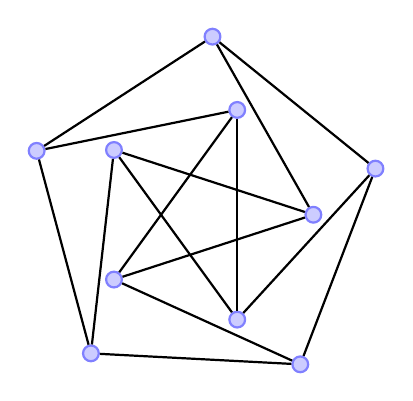
\begin{tikzpicture}[scale=1.4,vertex/.style={circle,draw=blue!50,fill=blue!20,thick,
        inner sep=0pt,minimum size=2mm}]
      \node[vertex] (inner1) at (1,0) {};
      \node[vertex] (inner2) at (72:1cm) {};
      \node[vertex] (inner3) at (144:1cm) {};
      \node[vertex] (inner4) at (-144:1cm) {};
      \node[vertex] (inner5) at (-72:1cm) {};
      \node[vertex] (outer1) at (15:1.6179cm) {};
      \node[vertex] (outer2) at (72+15:1.6179cm) {};
      \node[vertex] (outer3) at (144+15:1.6179cm) {};
      \node[vertex] (outer4) at (-144+15:1.6179cm) {};
      \node[vertex] (outer5) at (-72+15:1.6179cm) {};
      \path
      (inner1) edge [thick] node {} (inner3)
      (inner2) edge [thick] node {} (inner4)
      (inner3) edge [thick] node {} (inner5)
      (inner4) edge [thick] node {} (inner1)
      (inner5) edge [thick] node {} (inner2);
      \path
      (outer1) edge [thick] node {} (outer2)
      (outer2) edge [thick] node {} (outer3)
      (outer3) edge [thick] node {} (outer4)
      (outer4) edge [thick] node {} (outer5)
      (outer5) edge [thick] node {} (outer1);
      \path
      (inner1) edge [thick] node {} (outer2)
      (inner2) edge [thick] node {} (outer3)
      (inner3) edge [thick] node {} (outer4)
      (inner4) edge [thick] node {} (outer5)
      (inner5) edge [thick] node {} (outer1);
    \end{tikzpicture}
  \caption{Petersen's graph in $\R^2$ as a
    \href{http://en.wikipedia.org/wiki/Unit_distance_graph}%
     {unit-distance graph}.}
  \label{fig:pgf-petersen}
\end{figure}

\paragraph{Subfigures} Subfigures (that is, figures including several
``subfigures,'' as in \expref{Figure}{fig:sub-example}) can be produced with the
\lstinline.subcaption. package; this replaces the deprecated
\lstinline.subfigure. and \lstinline.subfig. packages. To use this
infrastructure, add
\begin{lstlisting}
\usepackage{caption,subcaption}
\end{lstlisting}
to the preamble of your document. Figures with subfigures are produced
as in the following example:
\begin{lstlisting}
\begin{figure}[ht]
  \begin{subfigure}[b]{.45\textwidth}
    \centering
    \includegraphics[width=2.5cm]{petersen}  %   An included image.
    \caption{Petersen's graph.}
    \label{subfig:Petersen}
  \end{subfigure}
  \quad
  \begin{subfigure}[b]{.45\textwidth}
    \centering
    (tikz picture code removed)
    \caption{Petersen's graph in $\R^2$ as a
      \href{http://en.wikipedia.org/wiki/Unit_distance_graph}%
        {unit-distance graph}.}
    \label{subfig:pgf-petersen}
  \end{subfigure}
  \caption{Two subfigures with captions.}
  \label{fig:sub-example}
\end{figure}
\end{lstlisting}

 With labels properly
included in the subfigures, references to them are automatically
handled correctly: the \LaTeX\ fragment
\lstinline.\expref{Figure}{subfig:Petersen}. produces the reference
\expref{Figure}{subfig:Petersen}.

\begin{figure}[ht]
\begin{subfigure}[b]{.45\textwidth}
  \centering
  \includegraphics[width=2.5cm]{petersen}  %   An included image.
  \caption{Petersen's graph.}
  \label{subfig:Petersen}
\end{subfigure}
\quad
\begin{subfigure}[b]{.45\textwidth}
\centering
    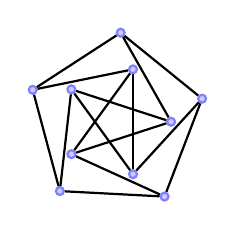
\begin{tikzpicture}[scale=0.7,vertex/.style={circle,draw=blue!50,fill=blue!20,thick,
        inner sep=0pt,minimum size=1mm}]
      \node[vertex] (inner1) at (1,0) {};
      \node[vertex] (inner2) at (72:1cm) {};
      \node[vertex] (inner3) at (144:1cm) {};
      \node[vertex] (inner4) at (-144:1cm) {};
      \node[vertex] (inner5) at (-72:1cm) {};
      \node[vertex] (outer1) at (15:1.6179cm) {};
      \node[vertex] (outer2) at (72+15:1.6179cm) {};
      \node[vertex] (outer3) at (144+15:1.6179cm) {};
      \node[vertex] (outer4) at (-144+15:1.6179cm) {};
      \node[vertex] (outer5) at (-72+15:1.6179cm) {};
      \path
      (inner1) edge [thick] node {} (inner3)
      (inner2) edge [thick] node {} (inner4)
      (inner3) edge [thick] node {} (inner5)
      (inner4) edge [thick] node {} (inner1)
      (inner5) edge [thick] node {} (inner2);
      \path
      (outer1) edge [thick] node {} (outer2)
      (outer2) edge [thick] node {} (outer3)
      (outer3) edge [thick] node {} (outer4)
      (outer4) edge [thick] node {} (outer5)
      (outer5) edge [thick] node {} (outer1);
      \path
      (inner1) edge [thick] node {} (outer2)
      (inner2) edge [thick] node {} (outer3)
      (inner3) edge [thick] node {} (outer4)
      (inner4) edge [thick] node {} (outer5)
      (inner5) edge [thick] node {} (outer1);
    \end{tikzpicture}
  \caption{Petersen's graph in $\R^2$ as a
    \href{http://en.wikipedia.org/wiki/Unit_distance_graph}{unit-distance
      graph}.}
  \label{subfig:pgf-petersen}
\end{subfigure}
\caption{Two subfigures with captions.}
\label{fig:sub-example}
\end{figure}
\section{Mathematical formul\ae{} and proofs}
\label{sec:math}

The AMS theorem class is loaded by default, along with standard macros
for many theorem-like environments. Theorems,
definitions, etc. are coded as follows:
\begin{lstlisting}
\begin{theorem}[Markov's inequality]
\label{thm:Markov}
  Let $X$ be a positive real-valued random variable.  Then, for
  every positive $\alpha$,
\begin{equation} \label{markov.eq}
  \Pr [ X \geq \alpha ] \leq \frac{E[X]}{\alpha}\,.
\end{equation}
\end{theorem}
\end{lstlisting}
The code above produces the following typesetting:
\begin{theorem}[Markov's inequality]
\label{thm:Markov}
  Let $X$ be a positive real-valued random variable.  Then, for
  every positive $\alpha$,
\begin{equation} \label{markov.eq}
  \Pr [ X \geq \alpha ] \leq \frac{E[X]}{\alpha}\,.
\end{equation}
\end{theorem}

Constructs for propositions, corollaries, claims, and lemmas are
predefined, invoked as above, and share numbering with theorems. For 
example:
\begin{lstlisting}
\begin{proposition}[Chebyshev's inequality]\label{prop:Chebyshev}
  Let $X$ be a real-valued random variable.  Then, for every positive
  $\lambda$,
  \[
  \Pr \bigl[ | X - E[X]| \geq \lambda \bigr] \leq 
  \frac{\sigma^2[X]}{\lambda^2}\,.
  \]
\end{proposition}
\end{lstlisting}
produces the following typesetting:
\begin{proposition}[Chebyshev's inequality]\label{prop:Chebyshev}
  Let $X$ be a real-valued random variable.  Then, for every positive
  $\lambda$,
  \[
  \Pr \bigl[ | X - E[X]| \geq \lambda \bigr] \leq 
\frac{\sigma^2[X]}{\lambda^2}\,.
  \]
\end{proposition}
\begin{sloppypar}
  Similar environments for definitions, conjectures, examples,
  remarks, and facts are also defined. They are typeset slightly
  differently but do share numbering with the constructs above. For
  example
\begin{definition}\label{def:stddev}
  Let $X$ be a real-valued random variable for which $E[X^2] <
  \infty$. The \emph{standard deviation} of $X$, denoted 
  $\sigma[X]$, is given by
  $$
  \sigma[X] = \sqrt{E\left[\bigl(X - E[X]\bigr)^2\right]}\,.
  $$
\end{definition}
If you wish to define a new theorem-like environment (\texttt{idea},
for example), you must inform \LaTeX\ about the environment in the
preamble of your document (that is, between the
\lstinline'\documentclass{toc}' command and the \lstinline'\begin{document}' 
command). If
  you wish to define the environment so that it is typeset like a
  Theorem (text in italics), use the sequence of commands:
\end{sloppypar}
\begin{lstlisting}
\theoremstyle{plain}
\newtheorem{idea}[theorem]{Idea}
\end{lstlisting}
If you wish to define an environment so that it is typeset like a
Definition (text in Roman), use the sequence of commands:
\begin{lstlisting}
\theoremstyle{definition}
\newtheorem{thought}[theorem]{Thought}
\end{lstlisting}
Proceed to use the construct in the body of your article as follows:
\begin{lstlisting}
\begin{idea}
  Use binary-coded-decimal instead of the long code.
\end{idea}
\end{lstlisting}
  This will produce the output:
\begin{idea}
  Use binary-coded-decimal instead of the long code.
\end{idea}
With the \texttt{thought} environment, the code will be this:
\begin{lstlisting}
\begin{thought}
  Use binary-coded-decimal instead of the long code.
\end{thought}
\end{lstlisting}
  This will produce the output:
\begin{thought}
  Use binary-coded-decimal instead of the long code.
\end{thought}

Proofs use the \lstinline`\proof` environment: the code
\begin{lstlisting}
\begin{proof}
  Expand the definition of $E[X]$.
\end{proof}
\end{lstlisting}
produces:
\begin{proof}
  Expand the definition of $E[X]$.
\end{proof}

In the case where a proof is not adjacent with the theorem it
supports, indicate this with the optional argument as below:

\begin{lstlisting}
\begin{proof}[Proof of \expref{Theorem}{thm:Markov}.]
  To prove inequality~\eqref{markov.eq}, expand the definition of
$E[X]$.
\end{proof}
\end{lstlisting}
produces
\begin{proof}[Proof of \expref{Theorem}{thm:Markov}.]
  To prove inequality~\eqref{markov.eq}, expand the definition of
$E[X]$.
\end{proof}

(We'll discuss the \lstinline`\expref` referencing command shortly.)

\paragraph{Equations.} Unnumbered equations,
like the one appearing in \expref{Proposition}{prop:Chebyshev} above, are
produced by the \lstinline'$$' (or \lstinline'\[' and \lstinline'\]') delimiters: for
example,
\begin{lstlisting}
$$
\sigma^2[X] = E\Bigl[\bigl(X - E[X]\bigr)\Bigr]\,.
$$
\end{lstlisting}
produces the equation
$$
\sigma^2[X] = E\Bigl[\bigl(X - E[X]\bigr)^2\Bigr]\,.
$$
Please use \lstinline'\,', as above, to provide space between
equations and any following punctuation. Note how the size of
delimiters such as $|$ and $[$ can be changed in an equation by use of
the modifiers \lstinline'\bigl' and \lstinline'\Bigl'. To have \LaTeX\
automatically adjust the size of such delimiters, use \lstinline'\left' and
\lstinline'\right', as in \eqref{eq:covariance} below.

Numbered equation are produced using the standard equation
environment. For example, the \LaTeX\ code
\begin{lstlisting}
\begin{equation}
  \label{eq:covariance}
  \cov[X,Y] = E\left[\bigl(X - E[X]\bigr)
    \bigl(Y - E[Y]\bigr)\right]\,.
\end{equation}
\end{lstlisting}
produces the equation
\begin{equation}
  \label{eq:covariance}
  \cov[X,Y] = 
       E\left[\bigl(X - E[X]\bigr)\bigl(Y - E[Y])\right]\,.
\end{equation}
To refer to
an equation from the main text body, use the \lstinline'\eqref' command
with the label attached to the equation by the \lstinline'\label'
command. For example, the reference equation~\eqref{eq:covariance} is
produced by the \LaTeX\ code
\lstinline'equation~\eqref{eq:example}'. (The \lstinline`~` produces a hard
space---\LaTeX\ will not allow it to break a line.)

\section{Labels and references}
\label{sec:refs}

\begin{sloppypar}
  Labels are attached to sections, theorems, equation and the like by
  invoking the command \lstinline`\label{labelname}` and usually referred
  to by using \lstinline`\ref{labelname}`. (See examples above.) Though not
  required by \LaTeX\ we suggest that label names follow a prefix
  convention that can used to identify the type of label. For example,
  labels attached to Theorems might be prefixed by \texttt{thm:}.
  This makes copy editing the \LaTeX\ file easier.
\end{sloppypar}

\begin{sloppypar}
Links will automatically be generated between references
like Theorem~\ref{thm:Markov} and the object to which they
refer. We provide an easy method to enlarge the size of the
hyperreference anchor, using the \lstinline`\expref` command. Specifically,
the command \lstinline`\expref{Theorem}{thm:Markov}` produces the
satisfactory output \expref{Theorem}{thm:Markov}. Please use
\lstinline`\expref` wherever you would use \lstinline`\ref`, with the exception
of equations, which are referred to with the \lstinline`\eqref` command:
\eg, \lstinline`equation~\eqref{eq:covariance}`.
\end{sloppypar}

\section{Bibliography; digital object identifiers}
\label{sec:bibliography}

The references you cite must be specified by a Bib\TeX\ database. As always with Bib\TeX, care must be taken to guarantee the correct appearance of author names (especially if they contain accents) and formulae appearing in titles. Consider the following two Bib\TeX\ entries, noting that portions of the Bib\TeX\ fields that must be processed verbatim by \LaTeX\ (\eg, for appearance of accents, math, and capitalization) are enclosed in braces:
\begin{lstlisting}
@article{v001a005,
 author = {Peter {H{\o}yer} and Robert {\v{S}palek}},
 title = {Quantum Fan-out is Powerful},
 journal = {Theory of Computing},
 year = {2005},
 pages = {81--103},
 doi = {10.4086/toc.2005.v001a005},
 volume = {1},
}

@article{v002a011,
 author = {Moses Charikar and Robert Krauthgamer},
 title = {Embedding the {Ulam} metric into {$\ell_2$}},
 journal = {Theory of Computing},
 year = {2006},
 pages = {207--224},
 doi = {10.4086/toc.2006.v002a011},
 volume = {2},
}
\end{lstlisting}

We will typeset your article with the Bib\TeX\ style file \texttt{tocplain.bst}, provided in the author kit. Please use this as you prepare your article for ToC; your bibliography (which appears before the \emph{about the authors} section) will be generated by the sequence of commands:
\begin{lstlisting}
...
\bibliographystyle{tocplain}
\bibliography{toc-example}
...
\end{lstlisting}

\paragraph{Digital object identifiers} Please provide a \emph{digital
  object identifier} (DOI) for those of your references that possess
them. These can be embedded directly in your Bib\TeX\ database using
the \lstinline`doi={}` field, as above. For example, the article
``Embedding the Ulam metric into $\ell_1$'' by \citet{v002a011}, which appeared in volume 2 of \textsl{Theory of Computing}, has been assigned the DOI:\href{http://dx.doi.org/10.4086/toc.2006.v002a011}{10.4086/toc.2006.v002a011}. In general, the DOI associated with an article can be found on the publisher's page for the article. For example, the DOI for the article ``Linearity testing in characteristic two,'' by \citet{BellareCHKS}, can be found on the \href{http://dx.doi.org/10.1109/SFCS.1995.492574}{article's homepage} on \href{http://ieeexplore.ieee.org/xpl/RecentIssue.jsp?punumber=18}{IEEE website for the IEEE Transactions on Information Theory}. The \href{http://www.informatik.uni-trier.de/~ley/db/}{DBLP} can be a fast way to find such article homepages.

\nocite{v001a005}

\bibliographystyle{plainnat}
\bibliography{toc-instructions}

\end{document}

%%% Local Variables:
%%% mode: latex
%%% TeX-master: t
%%% End:
